\documentclass[12pt]{article}
\usepackage{graphicx}
\usepackage{wrapfig}
\usepackage{subfigure}
\usepackage{multirow}
\usepackage{hyperref}
\usepackage{amsmath}
\usepackage{amssymb}
%\usepackage{ngerman}
\usepackage[ansinew]{inputenc}
\usepackage[left=2cm,top=1cm]{geometry}

% vector graphics test
\usepackage{color}
\usepackage{transparent}
\graphicspath{{graphs/}}

\usepackage{enumitem}
\setlength{\parindent}{0pt}



\begin{document}
	\pagestyle{empty}
	%\textasciitilde


\begin{titlepage}
    \centering
	\huge{Constructing the Equation of State for Compact Stars}\\
	\bigskip
    \large{Bachelor thesis}\\
    \huge{Jan R\"{o}der}
\end{titlepage}

%headline!!!


\tableofcontents
\pagebreak


\section{Introduction}

To this day, the nature of the equation of state [EOS] for neutron stars is highly debated. Previously discussed EOSs have emerged from
various topics and models of physics. Each one has different parameters determining its impact on calculations. \\
For the past years, it has been common to derive an EOS from a theory and then use it to construct a mass-radius relation [MRR]. This method is obviously constrained by the fact that one cannot put an arbitrary number of theories into one EOS. That would result in a problem impossible to solve, even for computers. Therefore, the motivation is to minimize the number of parameters and constraints in the future.\\
The approach chosen in this thesis is inverting the above process. Instead of using an EOS to calculate masses and radii, those shall now take over the role as input parameters. For compact stars up to a certain mass, the EOS will be assumed to be known well enough. Above that mass a numerical reconstruction will take place, determining the EOS from a variety of MRRs. 


\pagebreak
\section{Theoretical background}

\subsection{Compact stars}

At some point in a star's life, it is no longer capable of maintaining nuclear fusion in its core. Hydrogen burning first moves to a shell around the central region, further growing the previously produced helium core, up to the point where helium burning ignites. Depending on the star's mass, this process can either repeat until an iron core is formed or stop at some fusion product before that. In the latter case, i.e. for star masses up to $8$\,M$_\odot$, the outer envelopes will escape the core and form a planetary nebula. What remains is a white dwarf, with an upper mass limit given by Chandrasekhar as about $1.4$\,M$_\odot$. White dwarfs are the first known family of compact objects or -stars. Their interior structure depends on its progenitor star, hence their EOS is not universally defined (\cite{Glendenning}, p. 91). Their size is of order $10^3$\,km, temperatures usually reside in the $10^4$\,K domain but can be one or two orders of magnitude higher (\cite{Glendenning}, p. 90).\\
If the fusion processes have produced an iron core, it will be compressed to densities exceeding multiple times the nuclear saturation density when the star turns into a supernova explosion. The type of remnant left behind is called neutron star, and the matter out of which it is formed is always of the same composition and state. Therefore, in contrast to white dwarfs, there is one unique EOS to describe all neutron stars. \\
Both kinds of compact stars are subject to fast neutrino and photon cooling. After at most a few million years temperatures will have dropped several orders of magnitude below $1$\,MeV, so that on the nuclear scale the star can be  treated as cold. 

\subsection{Neutron star structure}

Generally, a neutron star can be divided into four zones: The inner and outer core, with inner and outer crust above it. These zones have fundamentally different properties. These zones are usually defined through their range of densities. For example, (one finds the original version of this proposal in \cite{Pandharipande1976} and \cite{ShapiroTeukolsky}), with $[\rho] =$\,g/cm$^3$:
\paragraph{$\rho\leq 10^6$} The \textit{surface} is the outermost region of the star, therefore temperature and and magnetic fields can have big impact on the equation of state here.
\paragraph{$10^6 \leq \rho \leq 4.3\cdot 10^{11}$} The \textit{outer crust} consists of a Coulomb lattice within a relativistic electron gas.
\paragraph{$4.3\cdot 10^{11} \leq \rho \leq (2-2.4)\cdot 10^{14}$} In the \textit{inner crust} neutron-rich nuclei from a lattice; as the densities increases, neutron drip takes place. Now, there is not only an electron gas, but also a superfluid neutron gas formed by the dripped-out neutrons.
\paragraph{$(2-2.4)\cdot 10^{14} \leq \rho \leq \rho_{core}$} The \textit{outer core} or \textit{neutron fluid} does no longer consist of a lattice. Remaining charge neutral, this region  
is dominated by a neutron superfluid along with a proton superfluid. The charge of the latter is evened out by electrons.
\paragraph{$\rho \geq \rho_{core}$} Within the \textit{inner core} lies the biggest mystery. One has no observational information about what processes happen at densities exceeding $10^{15}$\,g/cm$^3$. There are various theories about the state of matter in this region; possible are quark core formation or other types of phase transition.\\

The EOS becomes gradually less known towards the central region. A number of nuclear or fluid EOSs have been proposed, each including different aspects like interactions and states of matter, however it remains unclear how exactly a neutron star is built up. While a single EOS for the whole neutron star would be of great interest, one usually determines the EOS piecewise for each density region separately, imposing a phase transition between the layers. For a brief collection of models, see \cite{Pandharipande1976}.\\
The lack of information from direct measurement doesn't particularly improve this situation. However, for the first time, it might be possible to deduce information about the interior of a neutron star through data obtained by the NICER experiment located at ISS.


\subsection{The third family}

Most equations of state, plugged into the Tolman-Oppenheimer-Volkoff [TOV] equation (more on that in \ref{TOV}), will produce a relation between mass and radius [MRR] with a single maximum. From there on to lower radii the configurations become unstable due to a sign change in $dM/d\rho_c$ \cite{Harrison1965}. In 1966 Wheeler showed that, if the EOS was smooth, there would only remain a white dwarf and a neutron star branch in the MRR that would contain stable configurations. However, in 2000 Glendenning and Kettner discovered a class of EOSs that in contrast to Wheeler's work produced a third stable branch in the MRR \cite{GlennKett}. These stars would have the same masses as neutron stars (depending on the exact EOS, this might hold for a certain mass window) but significantly smaller radii. Therefore, one generally refers to these stars as "high mass twins" or "twin stars". 

\subsection{The Tolman-Oppenheimer-Volkoff equation} \label{TOV}

The equation used for determining the structure of compact stars will here be the TOV equation. To make analytical and numerical calculations easier, the unit system is chosen to be $c=G=1$, so that every unit is a 
power of length.\\
The derivation is based off the assumption that the star matter can be described as a perfect/ideal fluid. 
Further, the space-time shall not evolve in time, therefore staying spherically symmetric (i.e. it is stationary). In terms of the energy-momentum tensor we are left with:
\begin{equation}\label{eq:hydro}
	T_{\mu\nu}=\left(\epsilon + P\right)u_\nu u_\mu-Pg_{\mu\nu}
\end{equation}
Where $\epsilon$ is the energy density, $P$ is the pressure and $u_\mu$ is the 4-velocity. \\
Spherical symmetry leads to a certain form of the metric,
\begin{equation} \label{eq:line_element}
	ds^2 = e^{2\varPhi} dt^2 - e^{2\lambda}dr^2 - r^2(d\theta^2+\sin^2d\phi^2)
\end{equation}
containing spherical coordinates $r, \theta, \phi$ and a time-like coordinate $t$. Equation \ref{eq:line_element} becomes the line element for a flat space-time if the exponents in the first two coefficients become zero, from which follows the role of the exponent terms as curvature description in the radial and the time ``directions''. To be precise, $\varPhi$ is directly related to gravitational redshift, and $\lambda$ determines the change of proper length due to curvature.\\
This gives us the stress-energy tensor components:
\begin{equation}
	T_{\mu\nu} = diag(\epsilon e^{2\varPhi}  , \ P e^{2\lambda},\ Pr^2,\ Pr^2sin^2(\theta))
\end{equation}
One now imposes conservation of energy and momentum, 
\begin{equation}
	\nabla_\nu T^{\mu\nu}=0
\end{equation}
and puts it into the Einstein equations \ref{eq:einstein} together with the metric, the components of which can be read from \ref{eq:line_element}.
\begin{equation} \label{eq:einstein}
	R_{\mu\nu} - \frac{1}{2} g_{\mu\nu} R = 8\pi \,T_{\mu\nu}
\end{equation}
Here, $R_{\mu\nu}$ is the Ricci tensor and $R$ is the Ricci scalar. Both can be calculated from the metric $g_{\mu\nu}$. Before one can get to work to get the actual TOV equations, the metric exponential functions have to be calculated.\\
One obtains,finally, the full TOV equation:
\begin{equation}\label{eq:tov}
	\frac{dP}{dr} = \frac{(\epsilon + P)(m + 4\pi r^3 P)}{2mr-r^2}
\end{equation}
Together with a second equation for the mass:
\begin{equation}\label{eq:mr}
	\frac{dm}{dr} = 4\pi r^2\epsilon
\end{equation}


\subsection{Fermi gas equation of state}

% Glendenning, page???


This EOS will serve as a test case for the reconstruction algorithm (the constant in the polytrope will be set arbitrarily when using it as a first test). For a detailed version of this derivation, see \cite{Glendenning}. \\
Here, $p=k$ ($c=1$) and therefore $E=\sqrt{k^2+m^2}$. With that, the energy density, pressure and density become:
\begin{align}
	\epsilon &= \frac{\gamma}{2\pi ^2}\int_{0}^{k_F} k^2\sqrt{k^2+m^2} \ dk \\
	p &=  \frac{\gamma}{6\pi ^2} \int_{0}^{k_F} \frac{k^4}{\sqrt{k^2+m^2}} \ dk \\
	\rho &= \frac{\gamma}{2\pi ^2}\int_{0}^{k_F} k^2 \ dk
\end{align}
Setting the chemical potential to $\mu = \sqrt{k_F^2+m^2}$ (the Fermi energy), the solutions to these integrals read
\begin{align} \label{eq:eorho_solved}
	\epsilon &= \frac{1}{4\pi^2} \left[  \mu k_F \left(\mu^2-\frac{m^2}{2}\right)-\frac{m^4}{2} \ln \left(\frac{\mu +k_F}{m}\right)   \right] \\
	p &= \frac{1}{12\pi^2} \left[  \mu k_F \left(\mu^2-\frac{5m^2}{2}\right)-\frac{3m^4}{2} \ln \left(\frac{\mu +k_F}{m}\right)   \right] \\
	\rho &= \frac{k_F^3}{3\pi^2} \label{eq:rho}
\end{align}
where $\gamma = 2$, the degeneracy factor for fermions due to spin orientation. The Pauli principle is therefore directly included. Charge neutrality can be imposed, and chemical equilibrium can be obtained as
\begin{equation}
	\mu_n = \mu_p + \mu_e
\end{equation}
with chemical potentials for neutrons, protons and electrons.\\
Numerically, it is convenient to calculate limits of equations \ref{eq:eorho_solved} - \ref{eq:rho} for the case of high and low densities, i. e. $k_F \gg m$ or $k_F \ll m$. Our test case EOS will resemble very low densities. Expanding \ref{eq:eorho_solved} in $k_F/m$ one obtains
\begin{equation}
	p\sim K\cdot \rho^{5/3}
\end{equation}
Which is a polytropic type of equation. By absorbing densities into the energy density, one can get
\begin{equation}
	p = K\epsilon^\gamma
\end{equation}


\subsection{Numerical solution}

\subsubsection{Method}

The TOV equations come in the form of a first-order ordinary differential equation system (ODE). In order to obtain sufficient precision, a 4th-order Runge-Kutta algorithm shall be used to solve said ODE. By looking at both equations, our ODE system is given in the form:
\begin{equation}\label{eq:ode}
	\dot{y}(t) = f(y(t), t)
\end{equation}
where $\dot{y}(t)$ is a two component "vector":
\begin{equation}
	\dot{y}(t) =  \left( \begin{array}{c}dP/dr\\dm/dr\end{array} \right)
\end{equation}
$f(y(t), t)$ then contains the right hand side of equations \ref{eq:tov} and \ref{eq:mr}. \\
Numerically, solving the ODE is achieved by approximation of a step $\tau$ in the function variable $t$ (in TOV, this is the radius $r$) with derivatives of the function that is the ODE solution ($y$). 
\begin{equation}
	y(t+\tau) = y(t) + \frac{1}{6} (k_1 + 2k_2 + 2k_3 + k_4)
 \end{equation}
with increments $k_i$:
\begin{align*}
	k_1 &= f(y(t),t)\cdot\tau\\
	k_2 &= f(y(t)+k_1/2,t+\tau/2)\cdot\tau\\
	k_3 &= f(y(t)+k_2/2,t+\tau/2)\cdot\tau\\
	k_4 &= f(y(t)+k_3,t+\tau)\cdot\tau
\end{align*}
All $k_i$ are of course also two component "vectors". \\
For simpler test versions of the code, it is convenient to reduce the RK4 algorithm to RK1, or Euler's method. Also, the step size does not have to be adaptive. That way, runtime efficiency can be adjusted.

\subsubsection{Adaptive step size}

In order to maintain a minimum level of precision, the program checks for the change in pressure resulting from one Runge-Kutta step. If said change is too large, the step size $\tau$ is varied by a factor and the Runge-Kutta step count is reduced by one. Upon repeating the step, the same check takes place, and if necessary another $\tau$ adjustion. If the check is successful, the program will accept the step result and proceed with the next one. 

\subsubsection{Implementation}

In the actual program (written in C), the left hand side of our ODE system is implemented as a two-dimensional array of form y[N][x]. 
N will be two, for the whole program, as we will not add other equations to the system. The $k_i$ are all one-dimensional arrays; that way $x$ is only reflecting the step count. $x$ will therefore be in range zero up to the number of iteration steps. We set an arbitrary maximum step amount to prevent segmentation faults.\\
The RK4 algorithm will be implemented so that it can be easily modified any time to another order of Runge-Kutta or even Euler.


\subsection{From TOV solver to reconstruction}

After implementing the TOV equations together with the integration method, one can now generate a MRR by looping over several $p_c$ and using one EOS only. This MRR will be used for testing the final reconstruction code, which will consist of the TOV solver extended with the reconstruction algorithm explained below.\\
The main additions will be the split of the pressure range into segments, each requiring their own part of the EOS, as well as a segment determining the ``correctness'' of calculated mass and radius. The code will work not as ``inversely'' as was proposed before; the stars will still be integrated from the core towards the surface. However, the reconstruction no longer uses one single EOS.


\subsection{The inverse problem}

The first one to propose an inverted approach to the so-called ``stellar structure problem'' was L. Lindblom in 1992 \cite{Lindblom(1992)}. The ``standard'' version of this problem is just an integration of the TOV equations with a set EOS and central pressure, determining the total mass and radius (values of the variables at the surface). Lindblom presents an MRR-EOS-pair to be uniquely linked by an abstract map. This gives rise to the possibility of using that map in the other direction, i.e. from MRR to EOS. His ``traditional'' solution of the inverse problem works as follows:\\
Instead of integrating the TOV equations from the core towards the surface with initial values $p=p_c$ and $r=0$, he uses $M=m(R_{surface})=m(R)$ and $R$ as starting point to the calculation. Also, Lindblom assumes the EOS to be known up to some pair \{$\epsilon_i, p_i$\} corresponding to a star \{$M_i, R_i$\}. Looking at the next star, \{$M_{i+1}, R_{i+1}$\} are set as initial values and integration takes place until \{$\epsilon, p$\} reach \{$\epsilon_i, p_i$\}. At this point, a core \{$m_{i+1}, r_{i+1}$\} is left to be integrated. By representing the TOV equations for this small region as a power series, and inverting that, one can obtain \{$\epsilon_{i+1}, p_{i+1}$\} as a function of previously calculated quantities. This algorithm is repeated for the rest of the MRR, using an interpolation method to link \{$\epsilon_{i+1}, p_{i+1}$\} to the known EOS.\\
Here, a different and more simplistic approach to this problem is developed. This new method does not require the star to be integrated from crust to core, but will merely be a modification of the standard problem. This leads to a kind of ``trial and error'' type of solution, as section \ref{recon_method_sec} will explain more detailed.




\section{Reconstruction method} \label{recon_method_sec}

\subsection{General goal}

The goal is to reconstruct the EOS with as few biasing and imposing of mathematical form as possible. Therefore, the only pre-determined input is an EOS corresponding to a given mass in the MRR (Fig. \ref{fig:mce}). From there, the EOS can be constructed without further constraint. Here, a straight line is added to the end of the EOS, that is, in the high density region (Fig. \ref{fig:recon} b). The ODE solver starts at a point near the end of the given EOS and will calculate a mass with the (now small) piece of straight line and the EOS. If the mass does not fit the corresponding one in the MRR that was read in previously, the starting point on the line will be shifted to a higher pressure by a small step. At some very high pressure, a cut-off can be applied due to un-physical energy densities. If the starting point reaches the cut-off and the correct mass was not found, the slope of the line is varied. The latter also happens when the radius that corresponds to the calculated mass does not fit the one corresponding to the radius in the file. in Fig. \ref{fig:recon} c) the slope and end point of the green line have been successfully varied and the next mass and radius are reconstructed using the variation of the red line. The green line is now a part of the given EOS. This process will be repeated until the end of the MRR file.
\begin{figure}
	\centering
	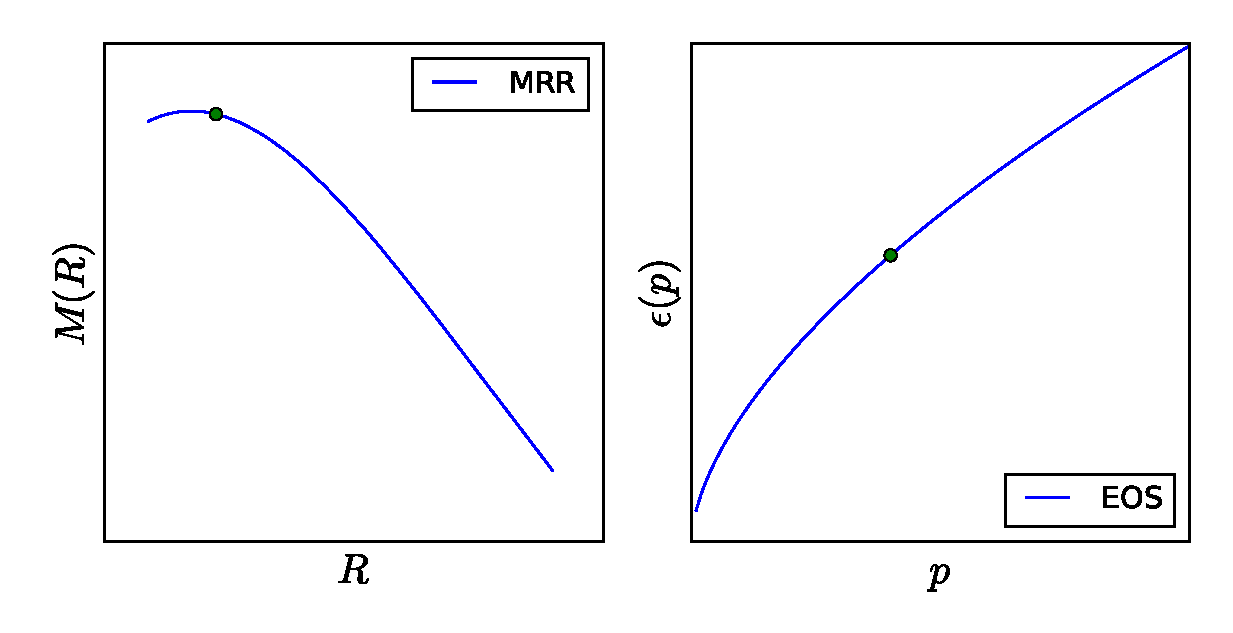
\includegraphics[width=1\textwidth]{graphs/mrr_corr_eos}
	\caption{corresponding points in MRR and EOS. Point in EOS resembles values in the center of the star.}
	\label{fig:mce}
\end{figure}
\begin{figure}
	\centering
	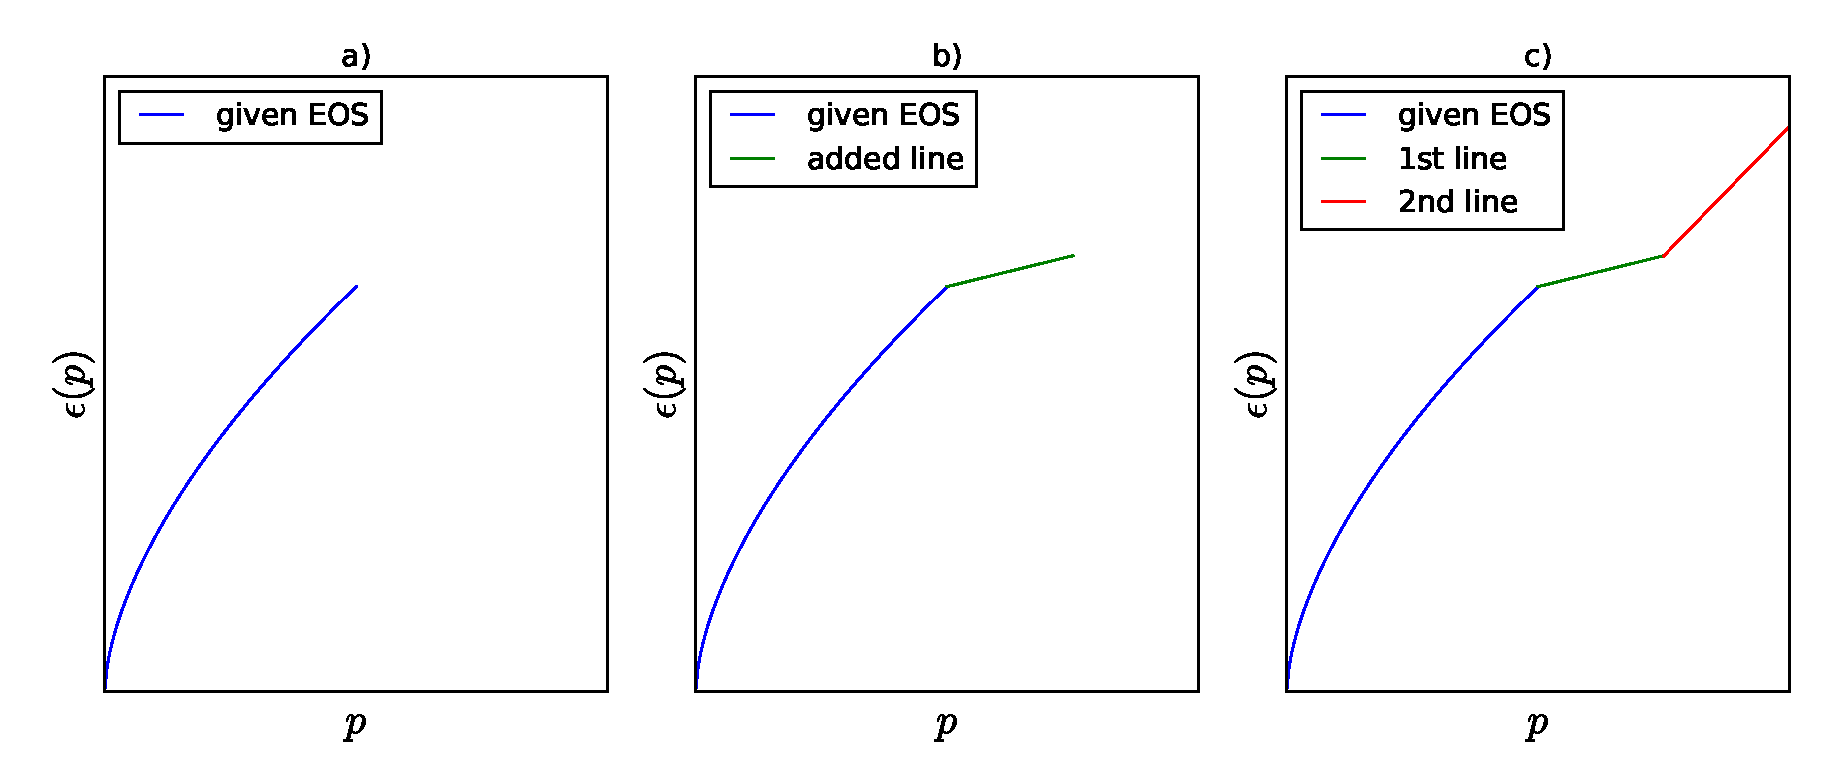
\includegraphics[width=1\textwidth]{graphs/eos_recon}
	\caption{a) Given polytropic equation of state, b) added a constructed straight line, c) Successfully varied green line, red line for next mass}
	\label{fig:recon}
\end{figure}


\subsection{Pressure intervals}

For the first mass in the file that is supposed to be reconstructed, the code will use the given EOS over the complete pressure interval $p_c$ to 0. That way, the first mass can be reproduced exactly in a test case. $p_c$ will be the last pressure value of the given EOS interval. From there, lines will be added to that end point; in the program, a flag labelled ``one'' will be set to false after the first mass was calculated. \\
From this point on it is important to determine which EOS will be used for what pressure interval inside the star. The second mass to be calculated will use the given EOS and one single line after it; masses number three and above then also need a line, but before finishing with the given EOS the previously determined lines are supposed to fill in the rest of the pressure range. \\
The line currently subject to variation will start at the central pressure ($p_c$) and will end at the last pressure a star was reconstructed for. This is resembled by the end point of the last previous line (or in the special case, the last pressure of the given EOS). The last given EOS pressure is saved in the very beginning as $p_{p_init}$, marking the point from which the given EOS will finish up the mass calculation.

\subsection{Test case}

The first code test will take place with a simple polytropic EOS such as
\begin{equation*}
	\epsilon(p) = \left(\frac{p}{10}\right)^{3/5}
\end{equation*}
Using the TOV solver, an MRR is generated. For this simple case, RK4 was reduced to Euler's method and the step size is not adaptive. The MRR seen in Fig. \ref{fig:test} will be the first one to be reconstructed. 
\begin{figure}
	\centering
	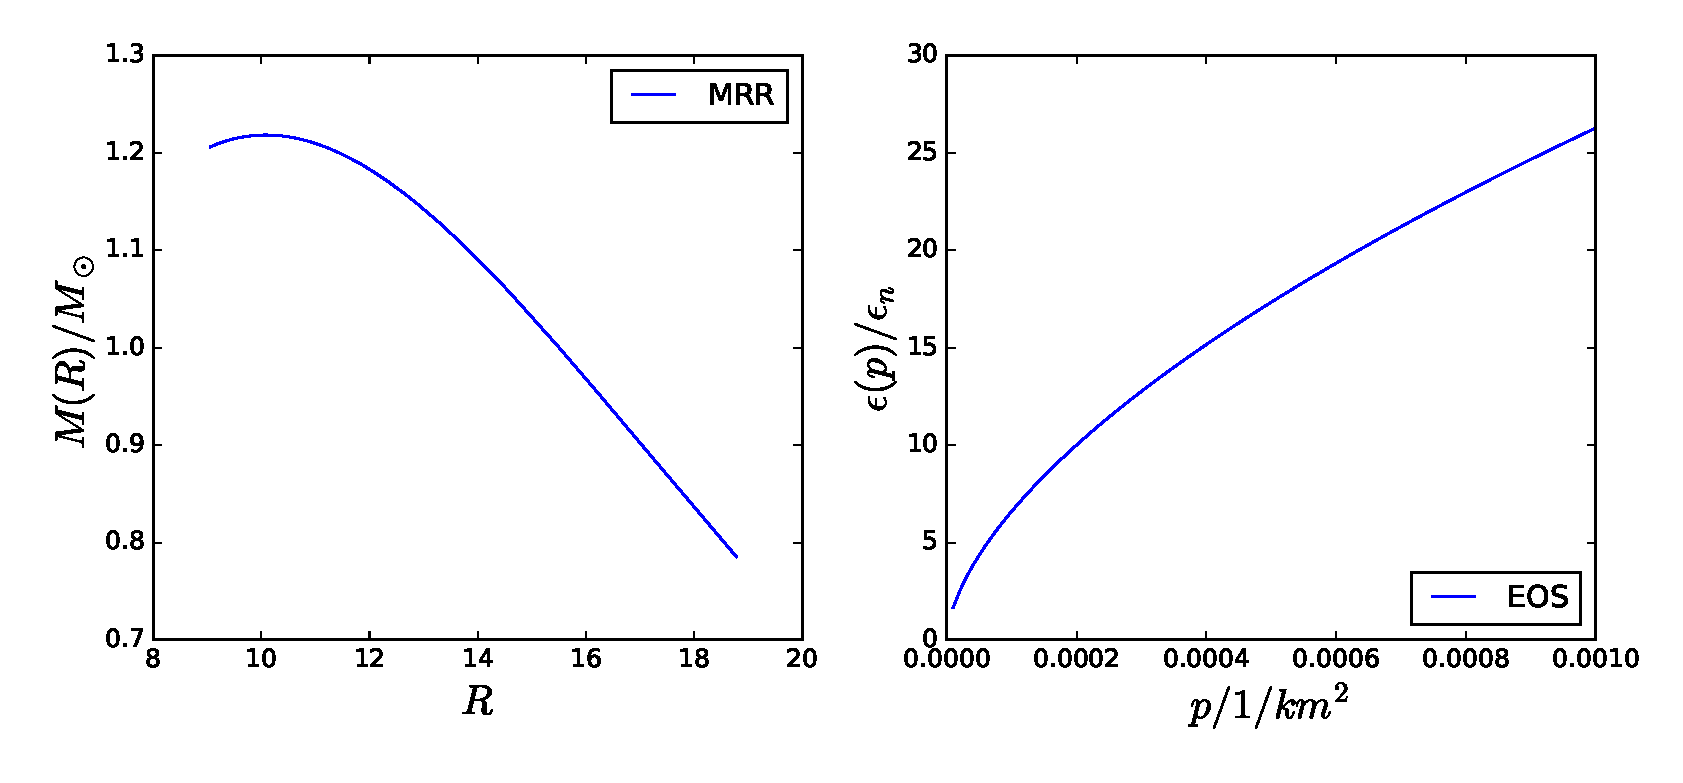
\includegraphics[width=1\textwidth]{graphs/test_mrr_eos}
	\caption{Test case}
	\label{fig:test}
\end{figure}
The curves both consist of 100 data points which will be read in by the reconstruction code. The result can be seen in \ref{fig:recon_test}.
\begin{figure}
	\centering
	\includegraphics[width=1\textwidth]{graphs/recon_test_mrr_eos}
	\caption{Test case}
	\label{fig:recon_test}
\end{figure}







\pagebreak
\pagebreak

%%%ALTERNATIVE BILDUMGEBUNG
% \begin{figure}[h]
% \begin{center}
% \includegraphics[width=50mm]{fig1}
% \caption{Fadenpendel \cite{Eichler}.}\label{fig:1}
% \end{center}
% \end{figure}




\hspace{15pt}

\begin{table}[h!]
  \centering
  %\caption{Caption for the table.}
  \label{tab:2}
  \begin{tabular}{|c||c|}
  \hline
    Messung der Fadenl�nge & $l$ (m)\\
    \hline\hline
    1 &   \\ \hline
    2 &   \\ \hline
    3 &   \\ \hline
    4 &   \\ \hline
    5 &   \\ \hline
    Mittelwert $\bar{l}$ &  \\ \hline
    Standardabweichung $\sigma_l$ &  \\ \hline
  \end{tabular}
\end{table}

%{1965gtgc.book.....H}
\begin{thebibliography}{2}
	\bibitem{Glendenning} Glendenning, N. K., Compact Stars: Nuclear Physics, Particle Physics, and General Relativity, Springer-Verlag New York, 2000, 1997
	\bibitem{Pandharipande1976} Pandharipande, V.~R., Pines, D., \& Smith, R.~A.\ 1976, Astrophys. J., \textbf{208}, 550 

	\bibitem{ShapiroTeukolsky} Shapiro, S.~L., \& Teukolsky, S.~A.\ 1983, Research supported by the National Science Foundation.~New York, Wiley-Interscience, 1983, 663 p. 252
	\bibitem{Harrison1965} Harrison, B.~K., Thorne, K.~S., Wakano, M., \& Wheeler, J.~A.\ 1965, Gravitation Theory and Gravitational Collapse, Chicago: University of Chicago Press, 1965
	\bibitem{GlennKett} Glendenning, N.~K., \& Kettner, C.\ 2000, A\&A, 353, L9 
	
	\bibitem{Lindblom(1992)} Lindblom, L.\ 1992, Astrophys. J., \textbf{398}, 569
	\bibitem{Haensel et al.(2007)} Haensel, P., Potekhin, A.~Y., \& Yakovlev, D.~G.\ 2007, Astrophysics and Space Science Library, 326, Haensel
	
%\bibitem{Eichler} H. J. Eichler, H.-D. Kronfeldt, J. Sahm, \textit{Das Neue Physikalische Grundpraktikum}, Springer-Verlag, Berlin-Heidelberg, 2001.
%\bibitem{Kuchling} H. Kuchling, \textit{Taschenbuch der Physik, 21. Auflage}, Fachbuchverlag Leipzig, 2014.
\end{thebibliography}

\end{document}